\newpage
\section{Szymon Jurecki - lover of useless facts}

\subsection{Pizza}
Let's suppose that a pizza has a radius equal z and height equal a. Then it's volume (V) is equal to:
\[V=Pi*z*z*a\]

\subsection{Random facts}
\begin{itemize}
    \item[!] The gap between two upper front teeth is called diastema.
    \item[!] The grey whale is not really grey. It's black.
    \item[!] There is a Historical Museum of Spaghetti in Pontedassio, Italy.
    \item[!] The pupil of an octopus's eye is rectangular.
    \item[!] Also known as the King of Hearts is the only king in the deck of cards, who doesn't have a moustache. 
\end{itemize}

\subsection{Bangladesh}
If you don't have anything interesting to do, i present to you demographic statistics of Bangladesh sorted according to it's divisions. I hope it helps you rethink your life decisions. (see Table~\ref{tab:bang})
\newpage
\begin{table}[h]
\centering
\begin{tabular}{|cc|c|c|c|}
\hline
\multicolumn{1}{|c|}{\textbf{Nr}} & \textbf{Division}                 & \textbf{Population}  & \textbf{Area}    & \textbf{Density} \\ \hline
\multicolumn{1}{|c|}{\textbf{1}}  & {\color[HTML]{000000} Barisal}    & 8 147 000            & 13 297           & 613              \\ \hline
\multicolumn{1}{|c|}{\textbf{2}}  & {\color[HTML]{000000} Chittagong} & 28 079 000           & 33 771           & 831              \\ \hline
\multicolumn{1}{|c|}{\textbf{3}}  & {\color[HTML]{000000} Dhaka}      & 46 729 000           & 31 120           & 1502             \\ \hline
\multicolumn{1}{|c|}{\textbf{4}}  & {\color[HTML]{000000} Khulna}     & 15 563 000           & 22 272           & 699              \\ \hline
\multicolumn{1}{|c|}{\textbf{5}}  & {\color[HTML]{000000} Rajshahi}   & 18 329 000           & 18 197           & 1007             \\ \hline
\multicolumn{1}{|c|}{\textbf{6}}  & {\color[HTML]{000000} Rangpur}    & 15 665 000           & 16 317           & 960              \\ \hline
\multicolumn{1}{|c|}{\textbf{7}}  & {\color[HTML]{000000} Sylhet}     & 9 807 000            & 12 596           & 779              \\ \hline
\multicolumn{2}{|c|}{\textbf{Bangladesh}}                             & \textbf{142 319 000} & \textbf{147 570} & \textbf{964}     \\ \hline
\end{tabular}
\caption{Administrative Divisions of Bangladesh}
\label{tab:bang}
\end{table}


.

\subsection{Striped cats}
Among the 19 pairs of chromosomes owned by every cat, there are 18 pairs called the autosomal chromosome and a pair of sex chromosomes. \textbf{Half of the sex chromosome pair is obtained from the male and the other half from the mother}. So a male cat will have 18 pairs of autosomal chromosomes and a pair of sex chromosomes \textbf{(X and Y; usually denoted XY)}, while a female cat has 18 pairs of autosomes and a pair of sex chromosomes \textbf{(X and X; denoted as XX)}.

The information about what color a cat will be is stored in the X sex chromosome. \textbf{Since female cats have two of them, if the colors on the chromosomes are not the same, \emph{the cat will be striped}} (see Figure~\ref{fig:cat}). On the other hand, \textbf{male cats have only one x sex chromosome} so there is only one color coded into their DNA and the cat will almost always have that color. In conclusion, \textbf{there are no striped male cats}.

\begin{figure}[t]
    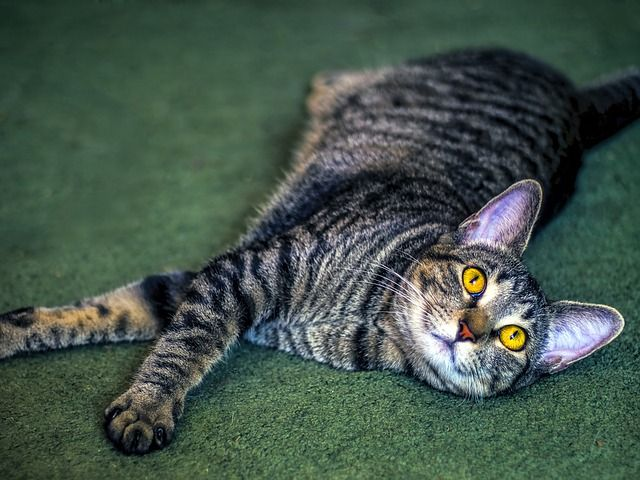
\includegraphics[width=10cm]{pictures/SzymonJ/cat.jpg}
    \centering
    \caption{Striped female cat}
    \label{fig:cat}
\end{figure}

\newpage
\subsection{Size of grapefruits}
List of possible sizes of a grapefruit from biggest to smallest:
\begin{enumerate}
    \item Big grapefruit
    \item Medium grapefruit
    \item Small grapefruit
\end{enumerate}